% GigaScience template
\documentclass[a4paper,num-refs]{oup-contemporary}

\journal{gigascience}


%%%% Packages %%%%
\usepackage{siunitx}
\usepackage{minted} % Used for JSON highlighting
\usepackage{algpseudocode} % Algorithmic environment
\usepackage{xspace}
\usepackage{booktabs}

%%%%%%

\usepackage{xcolor}
\usepackage{graphicx}
\usepackage{algorithm}
\usepackage{caption}
\usepackage{subcaption}
\usepackage{listings}
\usepackage{verbatim}
\usepackage{makecell}
\usepackage[flushleft]{threeparttable}

\usepackage{subcaption}
\usepackage{xspace}
\usepackage{stmaryrd} % for llbracket and rrbracket
\usepackage{amsmath}
\usepackage{ulem}
\usepackage{pifont}
\DeclareMathOperator*{\argmin}{argmin}



%%%% Commands %%%%
\newcommand{\todo}[1]{\color{red}\textbf{TODO:}#1\color{black}}
\newcommand{\note}[2]{\color{blue}Note: #1\color{black}}
\newcommand{\reprozip}[0]{ReproZip\xspace}
\newcommand{\tristan}[1]{\color{blue}\textbf{From Tristan:}#1\color{black}}
\newcommand{\english}[1]{\uwave{#1}}
\newcommand{\toolname}[0]{Spot\xspace}

 
\title{File-based localization of numerical perturbations in data analysis pipelines}
\begin{document}

\author[1]{Ali Salari}
\author[2,3]{Gregory Kiar}
\author[2]{Lindsay Lewis}
\author[2,3]{Alan C. Evans}
\author[1]{Tristan Glatard}

\affil[1]{Department of Computer Science and Software Engineering, Concordia University, Montreal, Canada}
\affil[2]{McGill University, Montreal, Canada}
\affil[3]{Montreal Neurological Institute, Montreal, Canada}

\maketitle

\begin{abstract} 

Data analysis pipelines are known to be impacted by operating system
updates and other infrastructural factors, presumably due to the creation,
propagation and amplification of numerical errors. However, the precise
causes of such instabilities and the path along which they propagate in the
pipelines are unclear, while this process could play a major role in the
current reproducibility crisis. We present a technique to identify the
computational processes in a pipeline that create numerical differences
when executed in different computational conditions. Our technique
leverages system-call interception to reconstruct processing and file
graphs without pipeline instrumentation. By applying our tool to the
structural pre-processing pipelines released by the Human Connectome
Project, we find that linear and non-linear registration are the cause of
most numerical instabilities in such pipelines, which confirms previous
findings. 

\end{abstract}

\begin{keywords}
Computational reproducibility; Numerical instability; Neuroimaging.
\end{keywords}


\section{Introduction}

% Reproducibility: crisis, numerical stability
% Containerization isn't the solution

Numerical stability is believed to play a central role in the differences
observed in data analysis pipelines across computational infrastructures.
Variability resulting from operating system upgrades, parallelization, or
even minor data perturbations may originate in errors that accumulate in
numerical computations, with important consequences on the reproducibility
of data analysis results. However, it remains challenging to identify the
exact elements in a complex pipeline that are prone to numerical instability,
leaving pipeline developers and users with the daunting task to manually
compare results obtained in different conditions. 

In neuroimaging, our primary application field, data analyses often consist
of hundreds of computational processes, sometimes coming from multiple
toolboxes, that are aggregated to perform a specific function. For
instance, the fMRIprep pipeline~\cite{esteban2019fmriprep} assembles software blocks
from FSL~\cite{jenkinson2012fsl}, AFNI~\cite{cox2012afni}, Freesurfer~\cite{fischl2012freesurfer} and ANTs~\cite{avants2009advanced} to provide a state-of-the art
functional MRI processing tool with minimal user input. Another example are the pipelines of the Human
Connectome Project~\cite{glasser2013} that combine tools from FSL and Freesurfer to pre-process
structural, functional and diffusion data from their
open dataset. In both cases, pipelines leverage toolboxes that are
widely trusted in the community. At the same time, substantial results
variations have been observed in these toolboxes resulting from minor data
or infrastructure perturbations~\cite{Glatard2015, Gronenschild2012, Lewis2017-ll}, which suggests that further investigation of their
numerical conditioning is required. For such complex pipelines, a
lightweight solution has to be found to perform such evaluations with
limited code instrumentation.

Numerical evaluations are traditionnally performed using techniques such as
interval arithmetics~\cite{hickey2001interval} that require complete code re-writes and are
therefore barely applicable to complex pipelines. Recently, Monte-Carlo
Arithmetic~\cite{Parker1997-qq, Denis2016-wo} provided a practical way to
evaluate the uncertainty of numerical results without the need to rewrite
the application in a different paradigm. By perturbating floating-point
computations, it introduces a controllable amount of noise in the
pipelines, effectively sampling results from a random distribution. While
this technique is very appealing, it suffers from two main issues that make
it impractical at the scale of a complete pipeline. First, it requires that
all software components be recompiled for MCA instrumentation, which is not
always feasible. Second, it multiplies the execution time by a factor of 10
to 100, which is impractical when executions already take a few hours to
complete. 

We present Spot, a tool to identify the source of numerical differences in
complex pipelines without instrumentation. Using system-call interception
through the Reprozip tool~\cite{chirigati2016reprozip}, Spot traverses graphs of processes and
intermediary files to pinpoint the pipeline components that are unstable
across execution conditions. When differences start accumulating,
effectively masking any further instability, it restores clean data copies
through a set of wrapper scripts. Wrapper scripts are also used to restore
temporary data that might have been deleted during the execution, and to
disambiguate files that have been written by multiple processes. The remainder of this paper 
presents the design of our tool, and its 
application to pre-processing pipelines of the HCP project. 

\todo{explain the issue with propagating differences and with transient files}

% % Verificarlo and MCA, require recompilation
% Numerical instabilities originate in the limited \todo{precision} of floating-point representations. 
% Traditionnaly, it has been evaluated through 

% % -> File-based analysis of pipelines without instrumentation
% % Reprozip

% Reproducibility is a crucial element of the scientific works, 
% as it enables researchers to evaluate authenticity and reliability 
% of the findings~\cite{plesser2018reproducibility}.
% Reproducibility is defined as the ability to regenerate the same 
% results as the original findings when the experiment is reanalyzed by 
% the same analytic methods, software package, parameters, and 
% data~\cite{peng2011reproducible}. 
% In addition, numerical reproducibility is defined as the ability to 
% regenerate bit for bit identical results from multiple 
% runs~\cite{hill2017numerical}. 
% We considered the numerical reproducibility in our experiments by comparing 
% the binary content of the results using the checksum method.

% Recently, validation of the reproducibility has been widely investigated 
% in the field of neuroimaging in which uses optimized 
% processing methods with the purpose of functional and structural 
% assessments of the human brain.
% According to the previous 
% studies, the variety of computing infrastructures including workstation 
% types, parallelization methods, operating systems, and analysis 
% packages are known to influence the reproducibility of the analyses~\cite{Gronenschild2012, 
% diethelm2012limits, Glatard2015, bowring2019exploring}.
% These irreproducibility issues are reported as the result of the 
% creation, propagation, and amplification of small numerical 
% differences.

% In particular, the effect of the operating systems on  
% computational pipelines shows the creation of small numerical differences~\cite{Glatard2015, Scaria2017}.
% These differences mainly correspond to the mathematical functions implemented 
% in different operating system libraries.
% For instance, changing the mathematical functions like \emph{expf()} and 
% \emph{cosf()} which manipulate the precision of floating-point representations, 
% between \emph{glibc} libraries in different operating systems can produce 
% small numerical differences.
% Besides, a similar issue is expected for any operating system which is 
% based on \emph{glibc}, the GNU C library.

% There are different approaches to improve the reproducibility of the analysis, 
% including containerization techniques that encapsulate software/hardware dependencies, 
% provenance capturing tools, and version control systems. 
% However, a comprehensive solution requires to fix the numerical instabilities instead of 
% masking the problem. For this purpose, bagging is one solution that has been used to 
% stabilize motion estimation analysis in fMRI~\cite{Glatard2018hbm}. 
% Bootstrap aggregation reduces the instabilities, but it needs expensive computations.
% As the second solution, a debugging tool can help to identify and 
% fix the instabilities in the pipeline. Therefore, we introduce 
% the numerical reproducibility measurement tool named \emph{Spot} to identify 
% the processes in the pipeline that create numerical differences across different conditions. 
% Furthermore, we can stabilize the identified processes in the next steps.

\section{Tool description}

The steps implemented in \toolname to compare pipeline executions in
2 conditions are outlined in Figure~\ref{fig:overview-tool}. First,
in Condition 1, a directed, rooted, bipartite provenance graph is built for
each subject, where nodes represent application processes or files, and
edges represent read or write file accesses (Step 1 in Figure~\ref{fig:overview-tool}). \emph{Transient} files are then identified as
 files that are either deleted during the execution, or modified by
multiple processes (Step 2). \toolname re-runs the pipeline to save these files
right after they are produced, resulting in a provenance \emph{DAG}
(Directed Acyclic Graph) in which file nodes have a single parent (in-degree
of 1) (Step 3). This DAG is then compared to the one produced from
Condition 2, in a step-by-step process that prevents the propagation of differences (step 4).
\toolname finally produces a labeled graph that identifies the
non-reproducible processes of the pipeline. 

\begin{figure*}
  \centering
    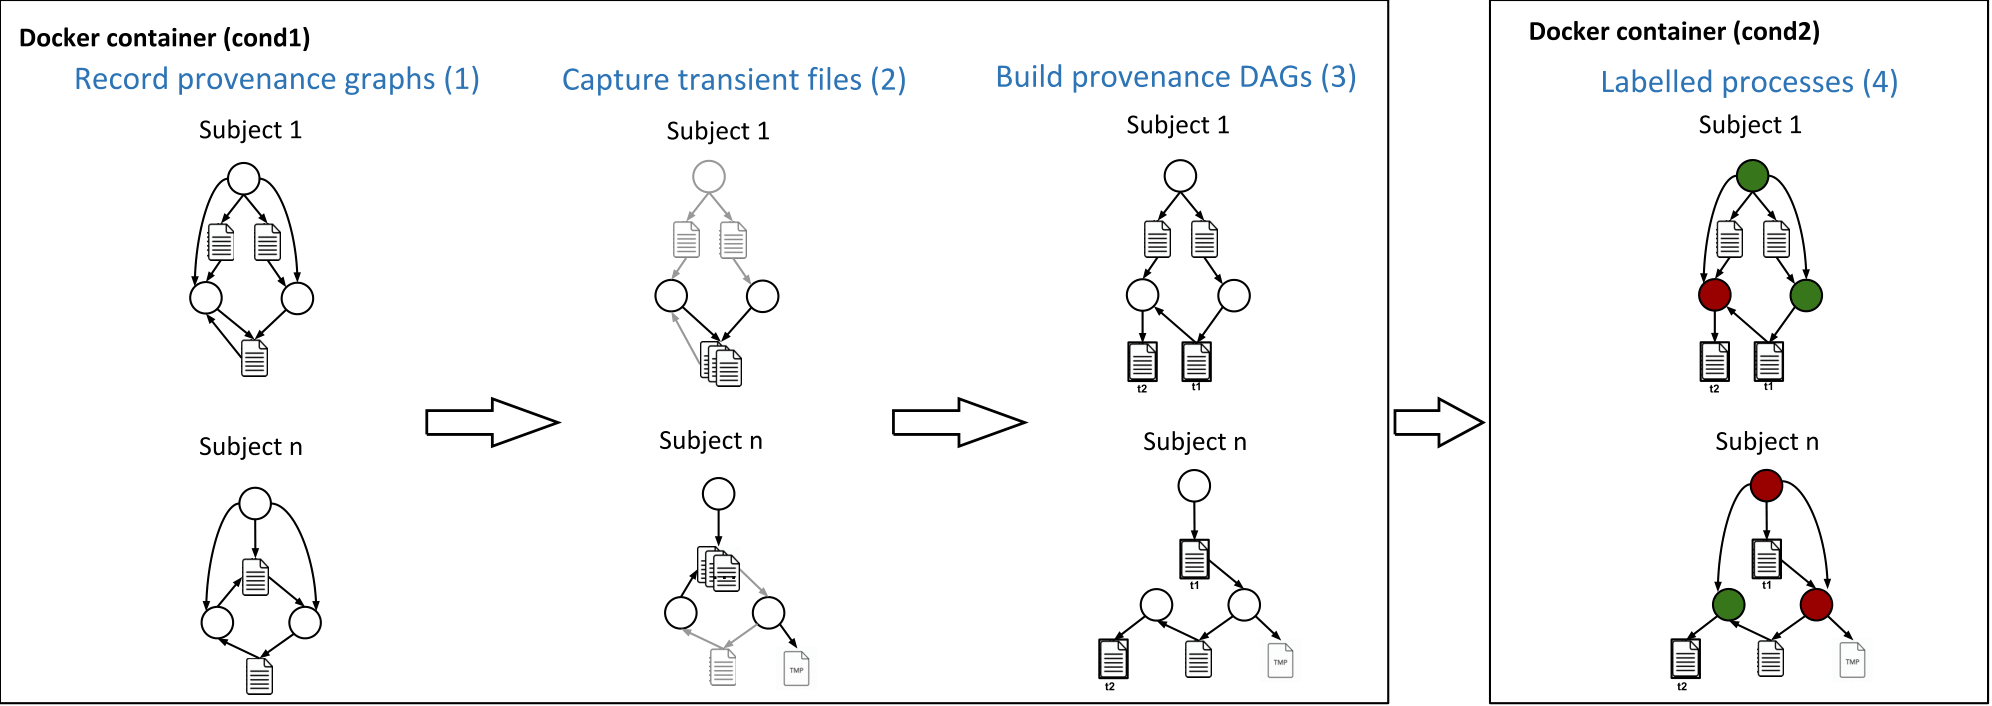
\includegraphics[width=.8\textwidth]{images/spot-diagram}
    \caption{An overview of Spot tool in four steps.
    (\href{https://docs.google.com/drawings/d/1OB3sB8kkK17Q516-TcmXKh3TwXSLDToJB11IVfUH5AU/edit?usp=sharing}{Source})}
    \label{fig:overview-tool}
  \end{figure*}


  \todo{review and summarize assumptions:
  * No concurrent writes from multiple processes
  * A given process cannot modify the bytes it wrote to a file
  * Process are command lines
  But we support non-concurrent writes by different processes. This is common in neuroimaging.
  }

\subsection{Recording provenance graphs}

We use the \reprozip tool~\cite{rampin2016reprozip}
to capture: (1) the set of processes created by the
pipeline, and
(2) the set of files read and written by each process, including
temporary files. \reprozip collects this information through the
\texttt{ptrace()} system call, with no required instrumentation of the pipeline.
\toolname then reconstructs a provenance graph by creating process and file
nodes from the \reprozip trace, and by adding directed edges corresponding
to file reads and file writes (Figure~\ref{fig:simple_script}-left). 

\todo{Is every process linked to an executable?}

Provenance graphs may be subject-dependent, which justifies the processing
of multiple subjects. For instance, data acquisitions may be
repeated a different number of times in each subject, for noise-reduction
purposes. Some of these differences can be neglected, for instance when a
data decompression step is present at the beginning of the execution for
some subjects only, but other differences cannot, for instance
when complete different processing paths are used in different subjects. 

\begin{listing}
  \inputminted{bash}{"bin/example.sh"}
  \caption{Example pipeline}
  \label{listing:sample-script}
\end{listing}

\begin{figure}
\centering
  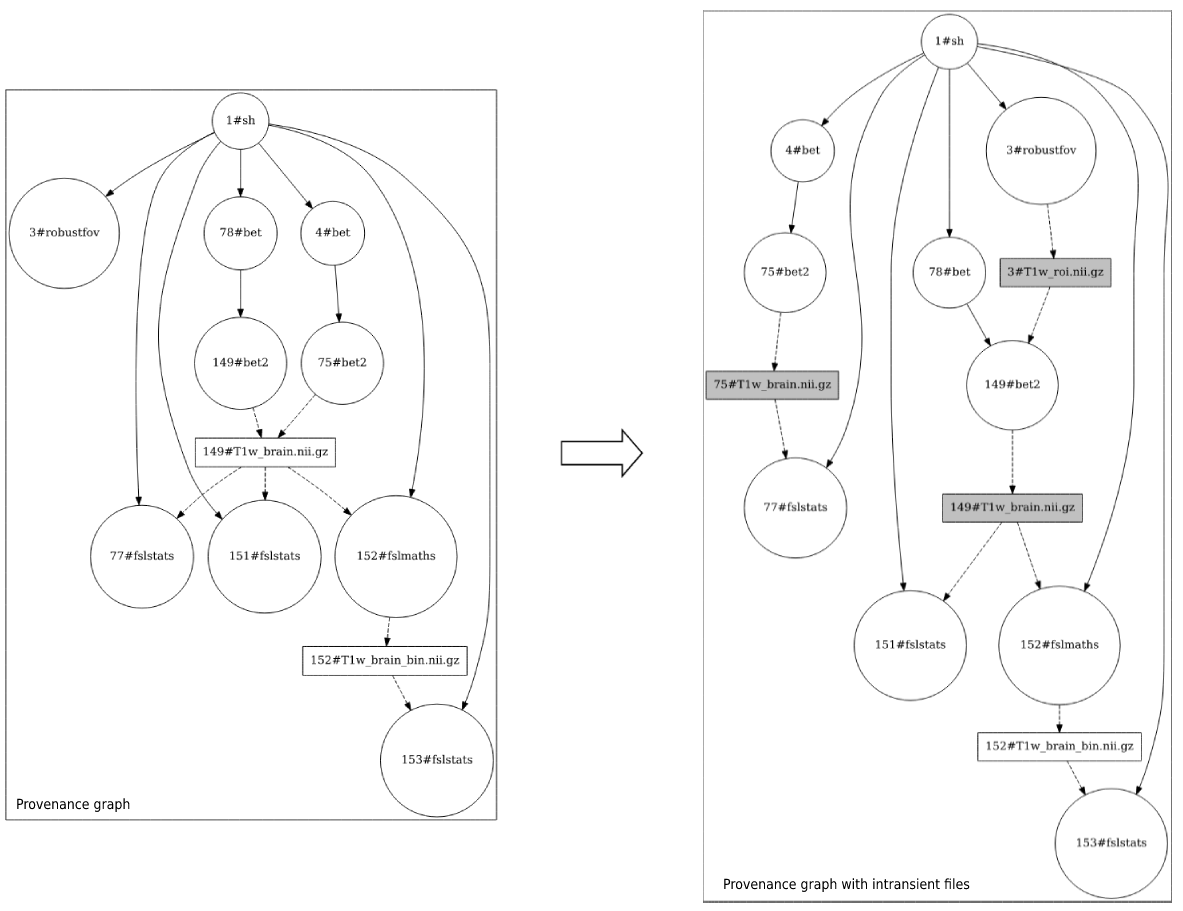
\includegraphics[width=1\columnwidth]{images/provenance-graphs}
  \caption{Provenance graphs
  constructed from the example pipeline in
  Listing~\ref{listing:sample-script}.
  Nodes are devided into two sets including processes that are shaped 
  in the circles and files that are shaped in the boxes.
  Transient files are represented with grey color boxes. 
  Plain edges 
  represent the process tree (\texttt{fork()} or \texttt{clone()} 
  system calls). Dashed edges represent file dependencies.
  Every node in the graph is labeled using (1) a process id created by our
  reconstruction, (2) the name of the executable run by the process or the file name.
  Process 0 is the initial call to the \texttt{sh} interpreter, and
  the rest of processes are the calls to FSL robustfov, bet, stats and maths made in
  Listing~\ref{listing:sample-script}. Processes 75 and 149 are forked by processes 4 and 78, respectively: 
  they were captured by \reprozip while they did not appear in
  Listing~\ref{listing:sample-script}.  
}
  \label{fig:simple_script}
\end{figure}

\subsection{Capturing transient files}

\toolname captures temporary files in Condition 1 by replacing every
process P by a wrapper that first calls P and then saves the produced
temporary files to a read-only directory. This process replacement is done
without pipeline instrumentation, by pre-pending to the \texttt{PATH} environment
variable a directory containing a wrapper script named as the executable
called by P.

Files written by multiple processes are disambiguated as follows. For a
 file F written by the processes in \textbf{P} = \{$P_{1}$, \ldots,
 $P_{n}$\}, \toolname first checks that processes in \textbf{P} do not
 write concurrently to F, which would violate our assumptions. Then, it
 replaces every process $P_{i}$ by a \texttt{PATH}-based wrapper that first
 calls $P_{i}$ and then saves F to a read-only directory. In this way,
 successive versions of F are preserved for comparison. \toolname finally
 updates the provenance graph accordingly, so that all files in the graph
 have an in-degree of 1 (Figure~\ref{fig:simple_script}-right). This operation also makes the provenance graph
 acyclic, since we assumed that a process can only write a single time to a file.

As an example, in the sample pipeline in
Listing~\ref{listing:sample-script}, process \texttt{3\#robustfov} writes a
temporary file. Also, file \emph{T1w\_brain.nii.gz} is first written
by \texttt{75\#bet2} and then overwritten by process \texttt{149\#bet2}. 
The complete list of the processes that
write transient files is captured in Listing~\ref{listing:json_process}.
Using this list, we modify processes in Condition 1 and then re-execute
pipeline to save them in a backup folder. 

\begin{listing}
  \begin{minted}[frame=single,
    framesep=3mm,
    linenos=false,
    xleftmargin=0pt,
    tabsize=4]{JSON}
{
  "multi_write_process": {
    "bet2\00T1w\00T1w_brain":
    {
      "files":[
        "/cond1/subj1/T1w_brain.nii.gz"
      ],
      "pid": 75
    },
    "bet2\00T1w_roi\00T1w_brain":
    {
      "files":[
        "/cond1/subj1/T1w_brain.nii.gz"
      ],
      "pid": 149
    }
  },
  "temp_process": {
    "robustfov\00-i\00T1w.nii.gz\00-r\00T1w_roi.nii.gz": 
    {
      "files": [
        "/cond1/subj1/T1w_roi.nii.gz"
      ],
      "pid": 3
    } 
  } 
}

\end{minted}
\caption{List of processes and transient files from the example pipeline in 
Listing~\ref{listing:sample-script}.}
\label{listing:json_process}
\end{listing}

\subsection{Labelling processes} 

Once all the files have been captured in Condition 1, including transient
ones, \toolname labels pipeline processes through a step-by-step execution
in Condition 2. Each process in Condition 2 is run and its output files are
compared to the ones produced in Condition 1. If no differences are found,
the process is marked as reproducible. Otherwise, the process is marked as
non-reproducible and the output files produced in Condition 1 are copied to
Condition 2, to ensure that differences do not propagate further in the
pipeline. Processes are instrumented transparently, through a modification
of the \texttt{PATH} variable similar to the one described previously. By
default, differences in output files are identified by comparing file
checksums. Other comparison functions can also be defined for specific file
types, for instance to ignore sections of the file containing timestamps or
other execution-specific information. Finally, \toolname creates a labeled
provenance graph, highlighting non-reproducible processes.

\begin{figure*}
  \centering
  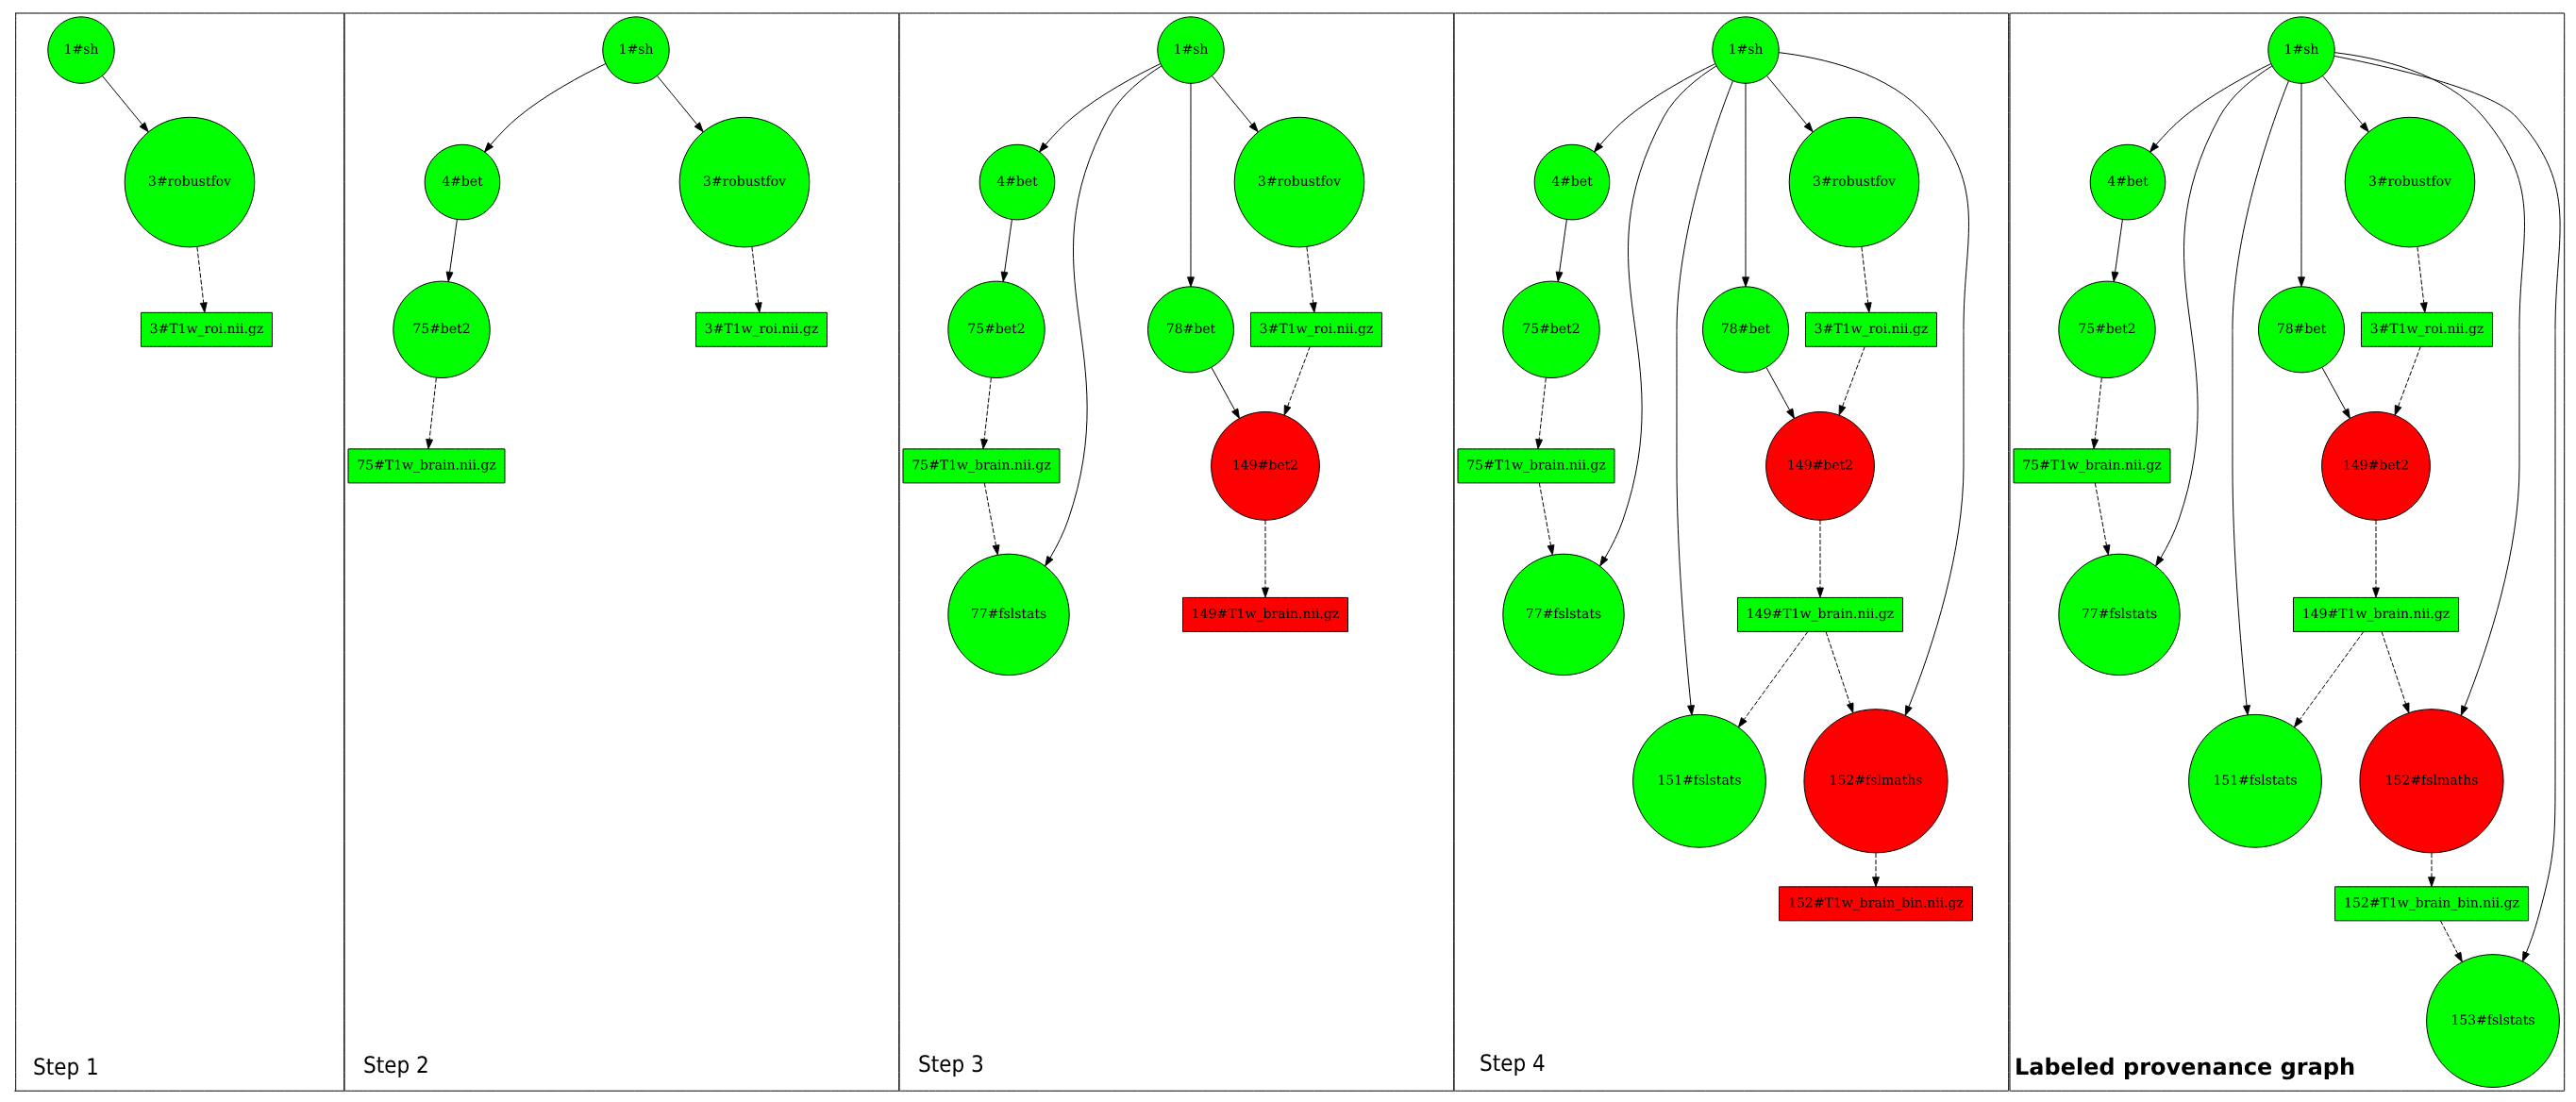
\includegraphics[width=.8\textwidth]{images/labelling-process}
  \caption{Illustration of the labelling approach. Non-reproducible processes are shown in red.}
  \label{fig:iterations}
\end{figure*}

Figure~\ref{fig:iterations} illustrates our incremental labelling 
process for the example in Figure~\ref{fig:simple_script}. 
At step one, process \texttt{3\#robustfov} is executed and then labeled 
as reproducible (green) as it produced files without differences.
At step 2, \texttt{75\#bet2} 
is also labeled as reproducible as it produced files without differences. 
At step 3 \texttt{149\#bet2} is labeled as non-reproducible (red) as it produced files with differences 
from files without differences. Therefore, the files produced by \texttt{149\#bet2} in  
Condition 2 are replaced with the files produced by \texttt{149\#bet2} in 
Condition 1.
At step 4, \texttt{152\#fslmaths} is labeled as non-reproducible as it writes files with differences.
At step 5, \texttt{153\#fslstats} is labeled as 
reproducible as the last process of the pipeline.

\section{Experiments}

In this experiment, we analyse the numerical reproducibility of computational pipelines 
and identify the origin of differences across the operating systems. 
Two types of differences can occur in the subjects due to the differences
in the operating systems. One is between-OS differences caused by the
operating system library updates and the other type, within-OS differences
occur as a result of the pseudo-random processes used in the pipelines.

In particular, Spot tool is tested on the neuroimaging applications which are 
predominantly using mathematical libraries. Therefore, we expect to find 
differences as a result of changing the mathematical functions between operating system libraries.

This section describes datasets and pipelines used for the analyses, and the way of data processing.

\subsection{HCP pipelines and dataset}

We used our tool to evaluate the reproducibility of the pipelines from the Human Connectome 
Project (\href{https://www.humanconnectome.org}{HCP}).
The HCP initiative is an effort to acquire and analyse 
brain connectivity data from 1200 healthy adults.
It enables the neuroscience 
research community to discover relationships between brain circuits and 
individual behaviors. This helps to understand a wide range of brain disorders.
The HCP project provides database services (ConnectomeDB) for storing and 
sharing primary and processed data freely, and data analysis pipelines that 
are available under an open-source license.

The HCP developed a set of pre-processing pipelines to process structural,
functional, and diffusion MRI data acquired in the project. We focus on HCP
pre-processing pipelines for structural data, particularly PreFreeSurfer
and FreeSurfer. 

According to~\cite{glasser2013}, the sequence of the 
sub-pipelines in PreFreeSurfer includes 
(1) Distortion Correction (DC), 
(2) Anatomical Average (AAve), 
(3) ACPC (Anterior Commissure, Posterior Commissure) Alignment (ACPC-A), 
(4) Brain Extraction (BExt), 
(5) Bias Field Correction (BFC), 
(6) Atlas-Registration (AR).

Also, the sequence of the main sub-pipelines in FreeSurfer includes 
(1) Downsampling images, 
(2) T1w image registration, 
(3) Placement of surface images, 
(4) Folding-based surface registration.
A detailed description of the analyses done in these
pipelines is available in~\cite{glasser2013}. 

Furthermore, the average time per subject taken for PreFreeSurfer processing is $\approx$ 2.2 hours, 
and FreeSurfer processing is $\approx$ 8.3 hours (20 runs), 
and the average output file size of 20 subjects in PreFreeSurfer is $\approx$ 2.7 GB, 
and FreeSurfer is $\approx$ 4.1 GB.

HCP data collected from different types of imaging techniques, including 
structural imaging (sMRI), functional imaging (fMRI), and diffusion imaging (dMRI).
The structural images include T1-weighted (T1w) and T2-weighted (T2w) images, which 
help in the diagnosis of brain injury.
The images are indexed with a suffix if several scans of the same modality were acquired.
For example, some data may include two T1w images with low and high resolutions.
The functional images, including task-based fMRI and resting-state scans, 
enable the measurement of functional activations within brain areas. 
Diffusion imaging is another kind of MRI technique, which measures 
the anatomical connectivity between regions.
See~\cite{van2013wu} for a discussion of these various modalities.

In this paper, we randomly selected 20 unprocessed subjects 
containing 3-tesla type of MRI scanners from the HCP data release S500 
available in \href{https://db.humanconnectome.org}{the ConnectomDB repository}. 


\subsection{Data processing}

We executed the pipelines using Docker containers to simplify the 
deployment of different operating system versions on execution 
platforms. 
The Docker images were built for the HCP pre-processing 
pipelines v3.19.0 (PreFreeSurfer and FreeSurfer) in 
CentOS 6.9 (Final) and CentOS 7.4 (Core). 
CentOS is a widely used operating system among the Neuroscience community because of 
the appropriate community support, network functions, safety, portability, and openness
~\cite{hanke2011neuroscience}.
These containers were installed with all the necessary software and libraries 
required to run the HCP pipelines including FSL (version 5.0.6), 
FreeSurfer (version 5.3.0-HCP, CentOS4 build), and Connectome Workbench (version 1.0).
Docker images are available on 
\href{https://hub.docker.com/r/bigdatalabteam/hcp-prefreesurfer/}{DockerHub}
for reuse.

The data were processed with PreFreeSurfer and FreeSurfer. 
First, PreFreeSurfer was utilized to analyse the unprocessed data, and then its 
results were used as the input of FreeSurfer.
Each subject was processed twice on the same operating system to detect
variability coming from pseudo-random operations. 
Within-OS variability may also be coming from other factors than pseudo-randomness. 
For instance, the same files may have different metadata such as timestamps, 
file paths, and other execution-specific information. 
To ensure that the differences are not related to the metadata, 
we used specific functions from FreeSurfer tool including 
\emph{mri\_diff}, \emph{mris\_diff}, and \emph{lta\_diff}.
These functions compare files based on the image dimensions, 
voxel intensities, the number of vertices, and geometry information
(see~\cite{fischl2012freesurfer} for more details). 
In addition, we used the Dice coefficient metric to evaluate the similarity of 
the image segmentation results, which is defined by
\[DICE=\frac{2(|X|\cap|Y|)}{|X|+|Y|}\]
The Dice coefficient ranges from 0, indicating X and Y have no voxels in common, to 1, if 
two images are identical. 

Finally, to cluster the subjects, the threshold value is set to zero in the clustering method. 
Also, we used the nearest neighbor algorithm to calculate the distance between clusters.


\subsection{Results}

% \subsection{Subject clustering}

% To reduce the number of provenance graphs to be examined, we cluster
% process trees using agglomerative hierarchical clustering, as implemented
% in SciPy~\cite{oliphant2007scipy}. We use the tree edit
% distance~\cite{zhang1989simple} between process trees, as implemented in
% the zss Python package. This distance is defined as the minimum number of
% edit operations to transform one tree into the other. Three edit operations
% are considered: node label modification, node removal, and node insertion.
% Each operation has an associated cost of 1. 
% //If threshold is 0, why do we even need the edit distance?//


\subsubsection{Within-OS differences}

We did not observe any within-OS difference in PreFreeSurfer, however, we
identified two FreeSurfer processes leading to within-OS differences due
to the use of pseudo-random numbers: image registration with
\emph{mri\_segreg}, and cortical surface curvature
estimations with \emph{mris\_curvature}. To address this issue, we fixed
the seed used by the pseudo-random number generator, through defining 
option ``--seed'' in the command-line of the processes.
Our analysis can focus on between-OS differences. 

\subsubsection{Between-OS differences in PreFreeSurfer}
%\subsubsection{PreFreeSurfer pipeline analysis} 

We identified four types of subjects with different PreFreeSurfer process
trees (Table~\ref{table:data-clusters}). Differences between subject types
are coming from different  numbers of T1 and T2 images in the raw data:
subjects of type 1 have 2 T1 images and 2 T2 images, while subjects of type
2 only have 1 T1 image and 1 T2 image. This leads to
different sets of output files. We verified that the process trees were
identical for all subjects of the same type, for both versions of
CentOS.

\begin{table}
\centering
\begin{threeparttable}
\caption{Clustering of 20 input subjects.}
\label{table:data-clusters}

\begin{tabular}{cccccc}
\toprule
       &                        &  \multicolumn{4}{c}{Available Modalities}    \\ 
\cmidrule(lr){3-6}       
Type   &   \makecell{Number of \\ Subjects}   &  T1w\_1          & T1w\_2      & T2w\_1          & T2w\_2        \\ \midrule
1      &               9                      &   \ding{51}      &   \ding{51} &   \ding{51}     &   \ding{51}   \\ 
2      &               8                      &   \ding{51}      &             &   \ding{51}     &               \\ 
3      &               1                      &   \ding{51}      &             &   \ding{51}     &   \ding{51}   \\ 
4      &               2                      &   \ding{51}      &   \ding{51} &   \ding{51}     &               \\ 
\bottomrule
\end{tabular}
\begin{tablenotes}
     \small
     \item *Type refers to the topology type of the process tree of subjects.
\end{tablenotes}
\end{threeparttable}
\end{table}


Figure~\ref{fig:pfs_freq} shows the frequency at which  processes create differences 
in the pipeline, and how differences are distributed among sub-pipelines.
Differences were observed in linear registration 
with FSL FLIRT (in ACPC-Alignment, Brain Extraction, Distortion Correction, 
Atlas Registration), in non-linear registration with FSL FNIRT (in Brain Extraction 
and Altas Registration), and in image warping with FSL \emph{new\_invwarp} (in Brain Extraction 
and Atlas Registration). Differences were also observed in image mean 
computations with FSL maths  (in Anatomical Average). 

The results show two types of differences, between-process and between-subject.
Between-process differences occur when the same tool behaves differently in different process instances.
For example, 
FLIRT tool always produces files without differences in \emph{AAve} sub-pipeline but 
mostly creates different files in \emph{AAli} sub-pipeline.
Also, different frequencies show between-subjects variability.
Accordingly, the same process can be reproducible for some subjects but not for others. 
The similar findings in another study~\cite{bowring2019exploring} were reported 
the effect of between-subject differences on reproducibility.
% Between subject differences can be a result of different subject types. 
% For instance, the subjects contain two T1 images need more calculations 
% to produce an average image between them.


% make figure in two columns use {figure*}
\begin{figure*}
\centering
  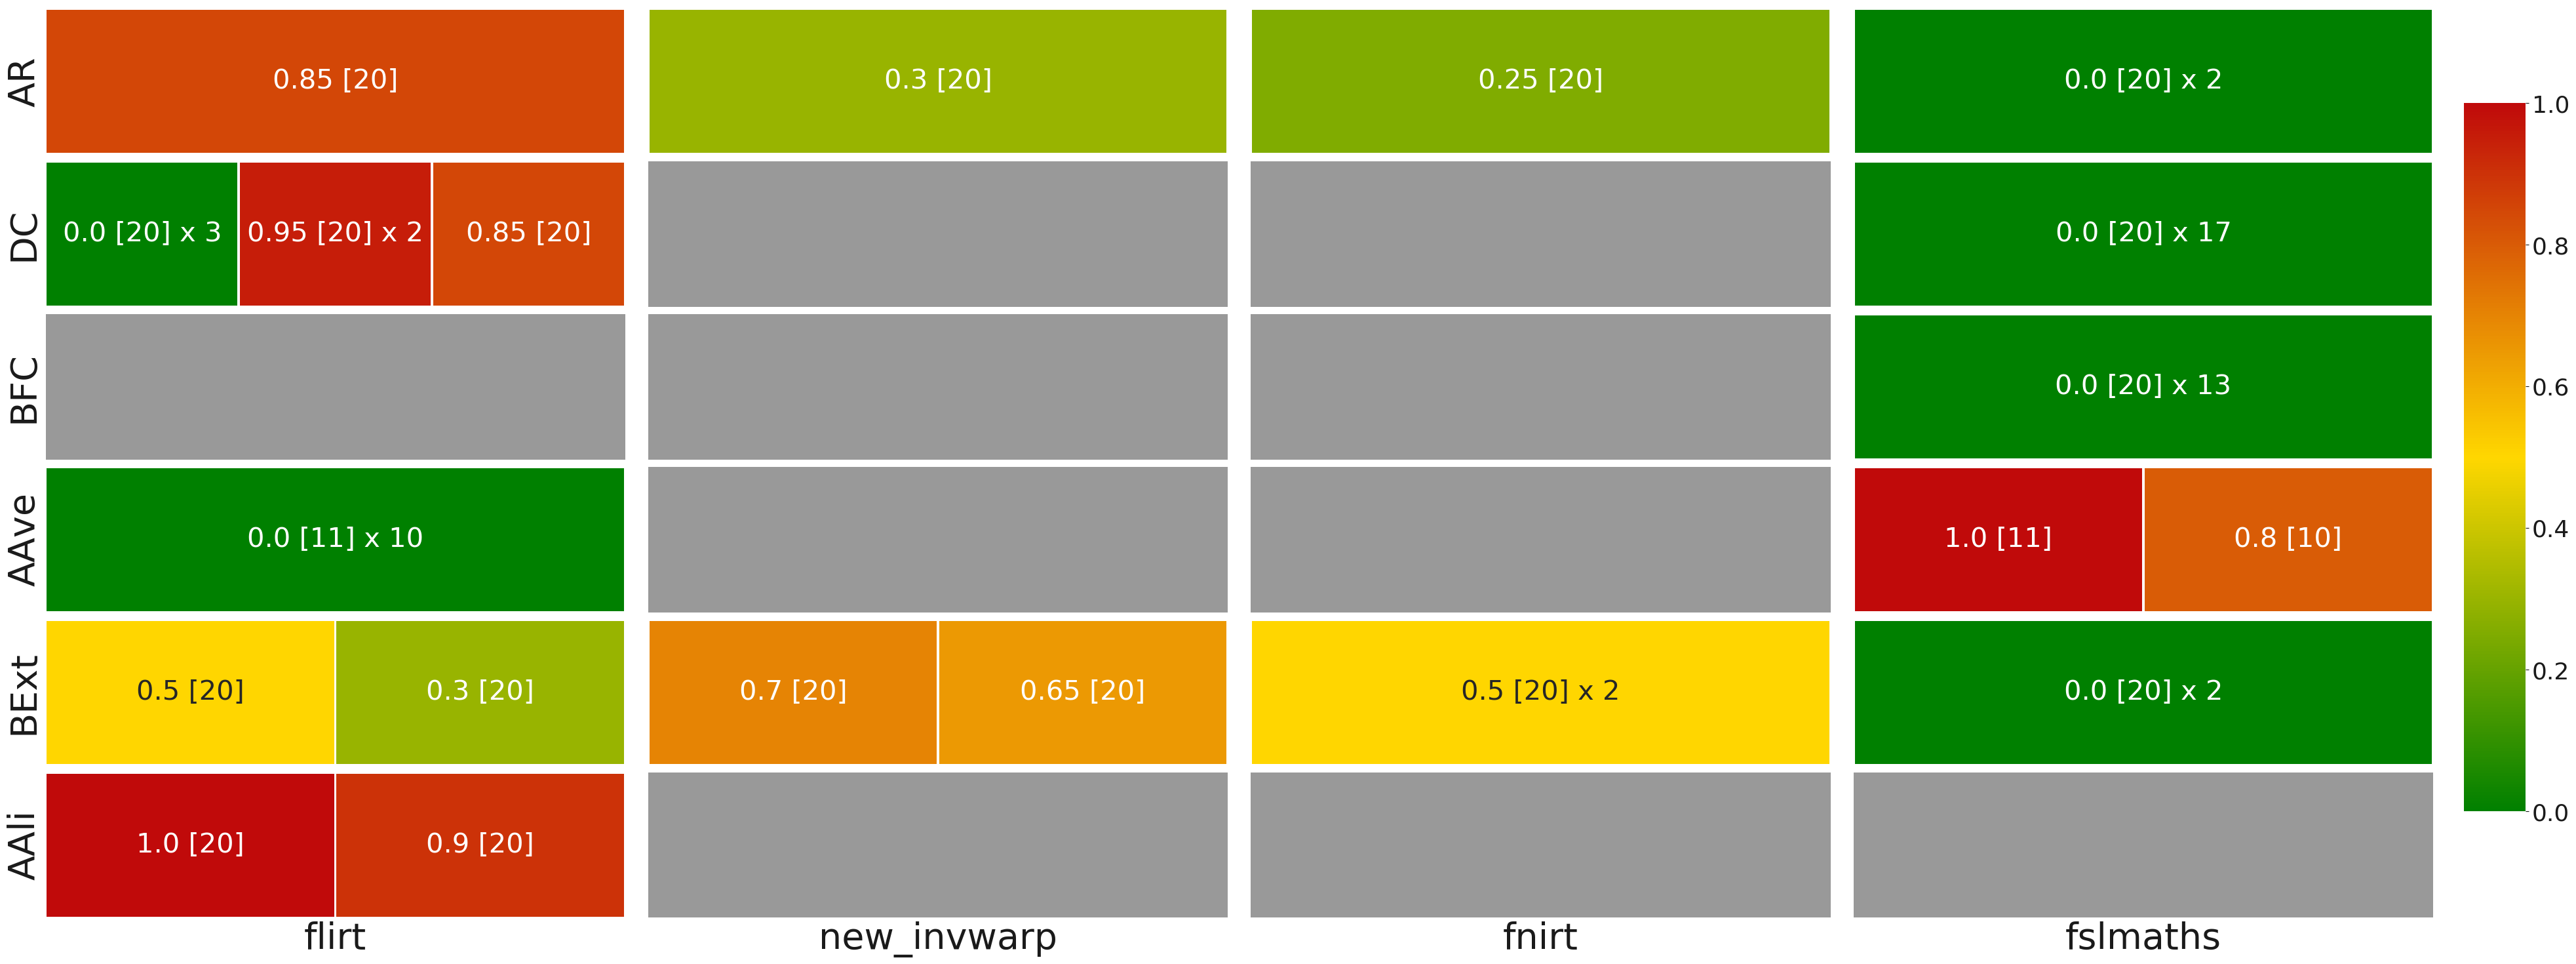
\includegraphics[width=\textwidth]{images/pfs_heatmap.png}
  \caption{Frequency heatmap of processes in the tools that introduce differences among 20 subjects. 
           Each column represents the pipeline tool, and each row shows the sub-pipeline.
           Each cell may contain several instances of the process of a tool in a sub-pipeline.
           Annotations describe the frequency distribution of the instances as ``N [M] x Y" 
           in which N is the proportion of the process 
           that creates differences out of all M times that is occurred. 
           Also, times Y shows the number of processes with the same distribution.
           For example, the cell of FLIRT tool in the sub-pipeline AAve shows 10 instances of the process 
           with the frequency of 11 that introduce no differences.
           The range between red and green colors shows the highest and lowest 
           proportion of occurrences of the processes with differences.
           Also, grey cells indicate that the tool is not executed in the sub-pipeline.}
  \label{fig:pfs_freq}
\end{figure*}


Figure~\ref{fig:fnirt_result} 
shows checkerboard image from the results of ACPC-Alignment in PreFreeSurfer. 
Each rectangle includes the replaced voxels with different intensity values between images.
The misaligned regions visually represent significant differences in the alignment 
procedure.

%Alternating rectangular regions between two images, creating a characteristic 
%checkerboard-like pattern of varying magnitudes.

\begin{figure}
  \centering
    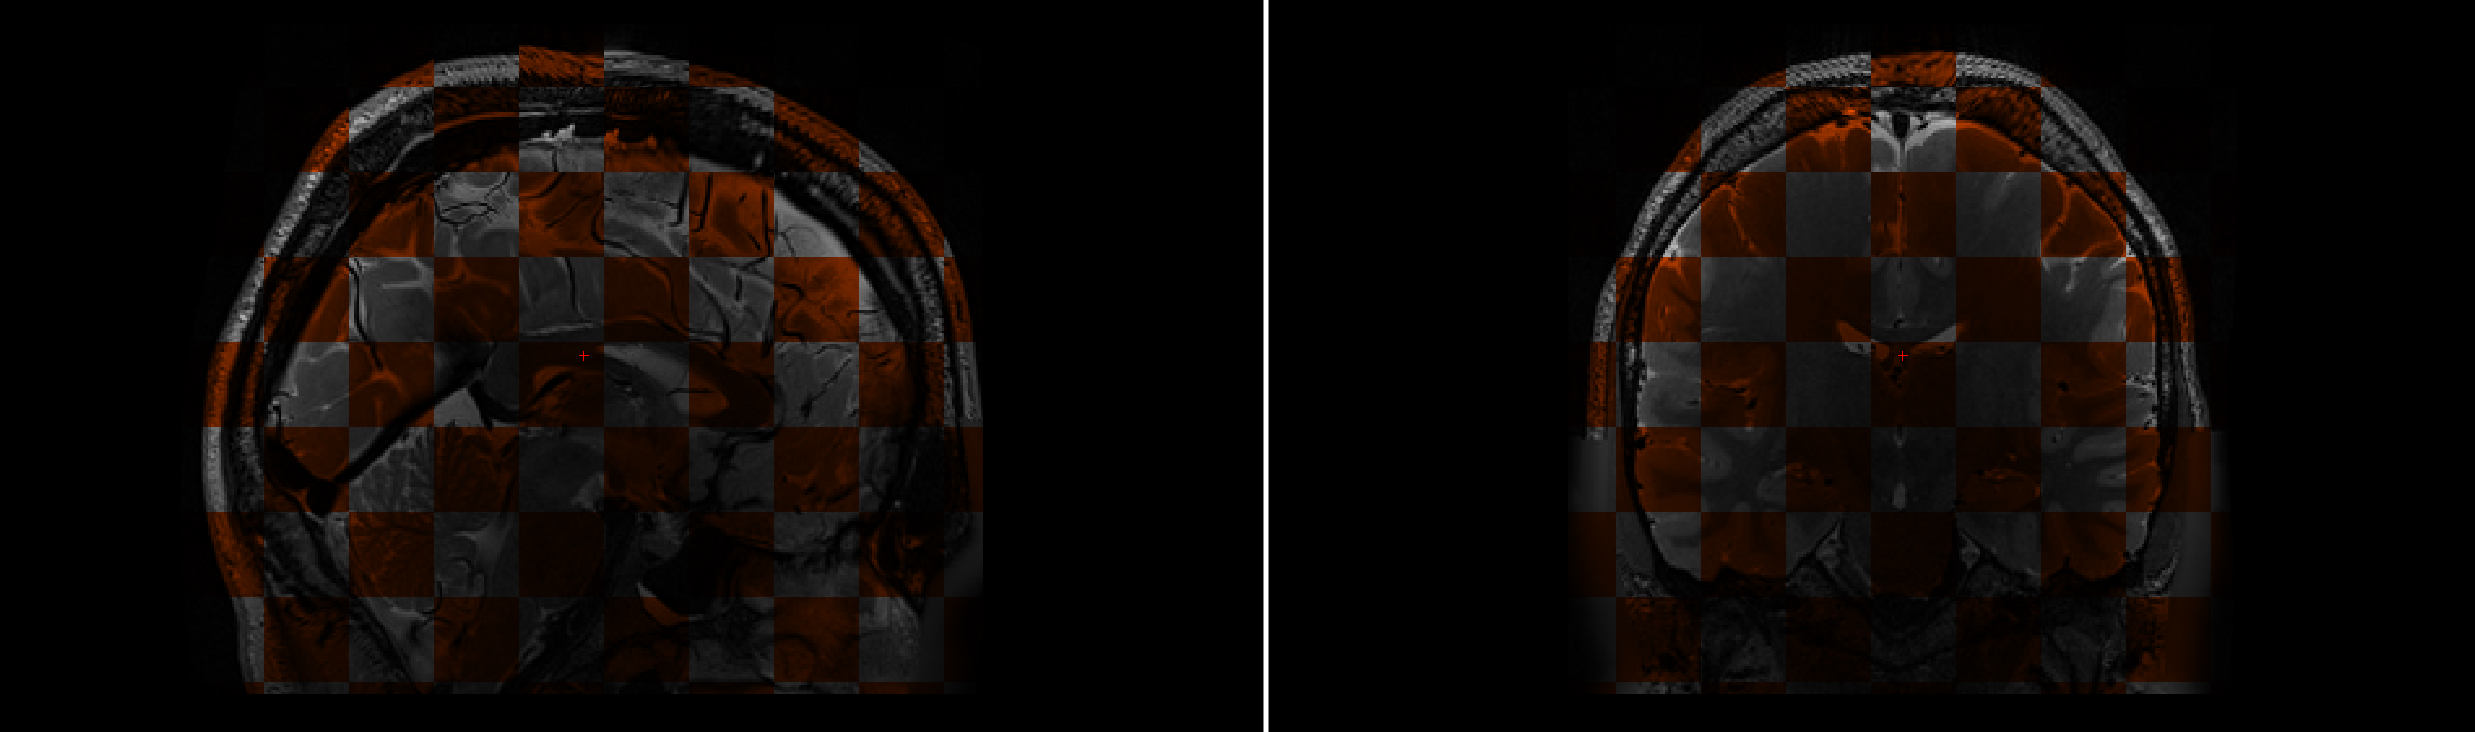
\includegraphics[width=\columnwidth]{images/t2w_alignment.png} 
    \caption{Differences between FNIRT results of one subject from PreFreeSurfer 
    (checkerboard image \emph{T2w\_acpc\_to\_MNI\_nonli.nii.gz}) (CentOS6 vs. 
    CentOS7).
    \href{https://github.com/ali4006/HCP-reproducibility-paper/blob/master/images/pfs_t2w_alignment.gif}
    {The link} to the animated version of alignment results shows the better visualization of differences.
} 
    \label{fig:fnirt_result}
\end{figure}


\subsubsection{Between-OS differences in FreeSurfer} 

We processed 20 subjects using FreeSurfer and 
Spot tool identified \emph{mris\_make\_surfaces} as the only process in 
the pipeline that creates differences in 10 subjects.
This process generates surface files for cortical and white matter surfaces 
(see~\cite{fischl2012freesurfer} for more detail). 
Also, FreeSurfer did not introduce any differences in 10 subjects. 

Results show that the static builds of FreeSurfer in which uses the embedded libraries 
significantly avoids the creation of differences.
However, we found that between-OS differences occur when pre-processed data are different in FreeSurfer. 
FreeSurfer may not introduce differences, but it propagates and amplifies 
the current differences that appeared in PreFreeSurfer results across the operating systems.

Figure~\ref{fig:tissue_class} illustrates the sum of binarized differences 
from 20 subject results of the brain tissue segmentation across OSes.
This figure shows between-OS differences  
as a result of the propagation and amplification of differences in FreeSurfer. 
Differences are mostly localized at the interfaces between tissues.
In our dataset, we found subjects with min Dice value of 0.89 and max Dice  
value of 0.96.

Furthermore, the scatter plots of the Dice coefficients of the 44 segmented regions obtained 
from two operating systems are shown in Figure~\ref{fig:scatter_plot}.
This figure shows high Dice coefficients (more than 0.95) in large regions and very low 
Dice coefficients (below 0.5) in small structures particularly in the vessels and lateral ventricles.


\begin{figure}
%  \includegraphics{brain\_classification}
\centering
  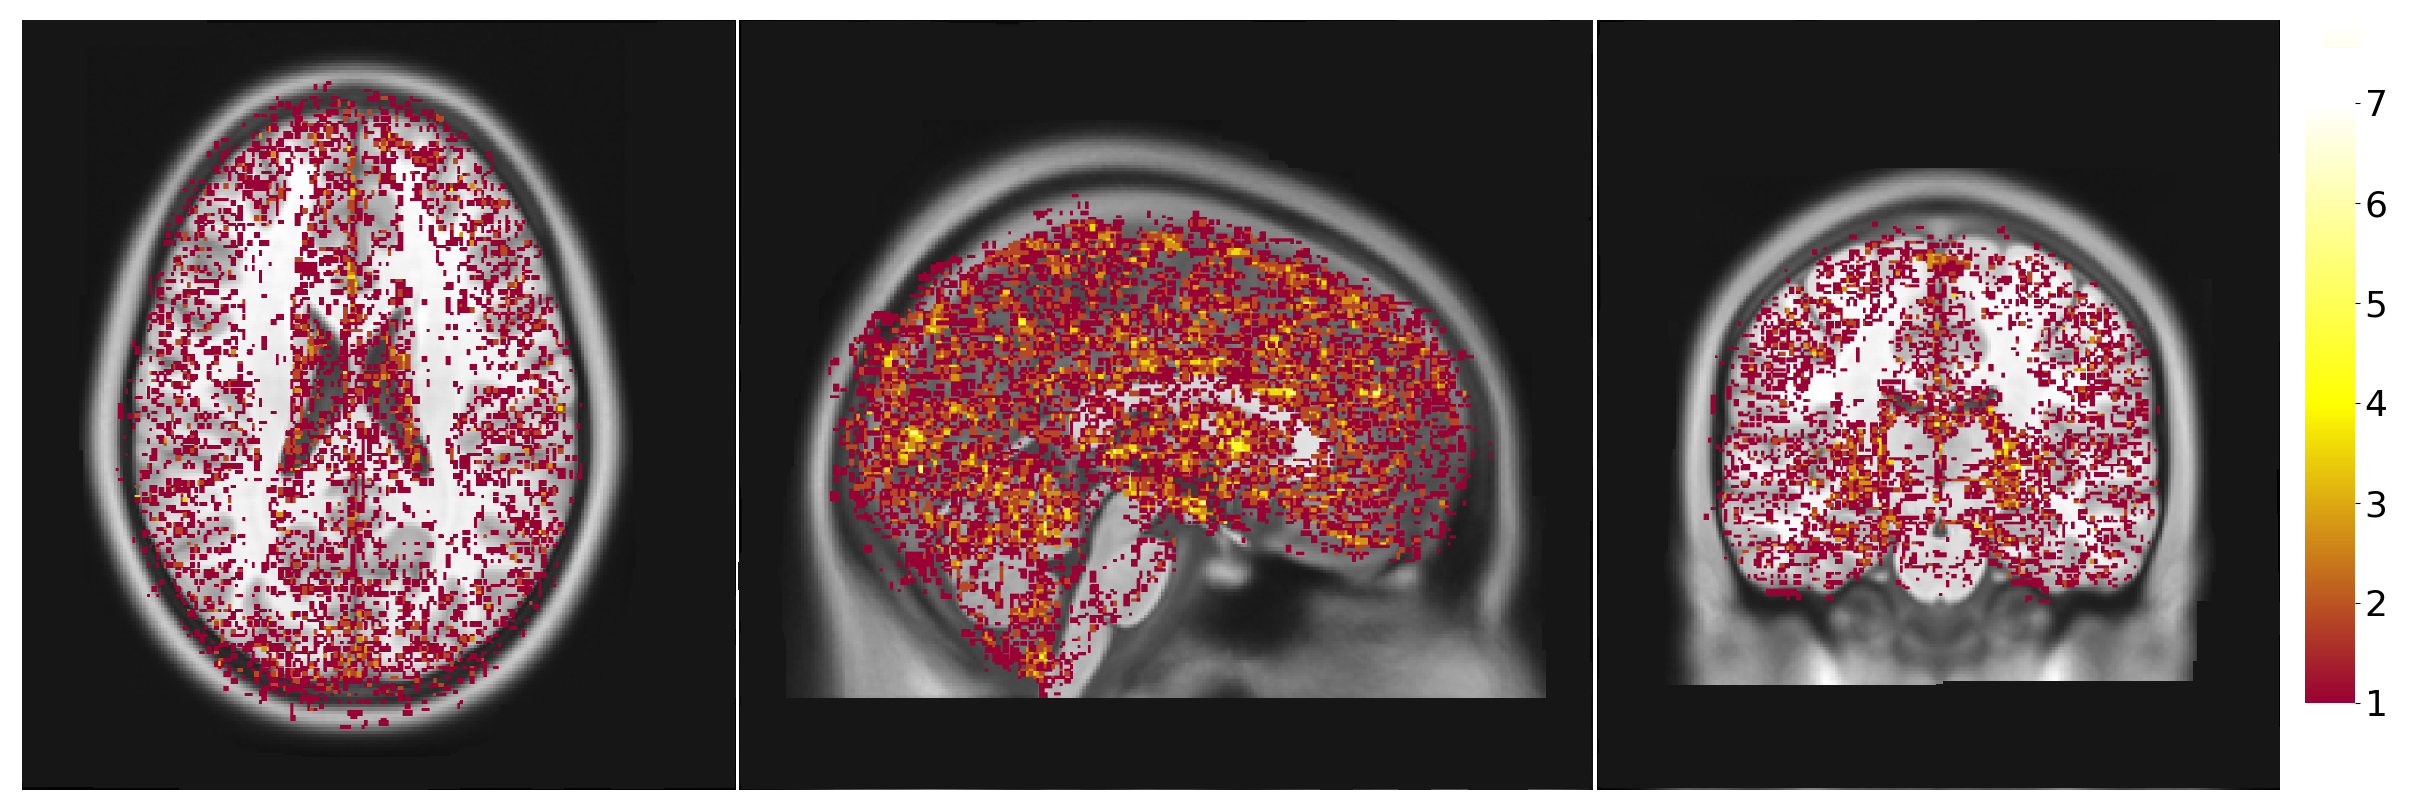
\includegraphics[width=\columnwidth]{images/brain_segmentation_mni.png} 
  \caption{Heatmap binarized differences between brain segmentation results (file \emph{aseg.hires.mgz}) from 
          20 subjects in FreeSurfer (CentOS6 vs. CentOS7). 
          All binarized differences were resampled to the default MNI152 volume template.
          \href{https://github.com/ali4006/HCP-reproducibility-paper/blob/master/images/fs_brain_segmentation.gif}
          {The link} to the animated version of segmentation results of one subject presents more clear illustration of differences.} 
  \label{fig:tissue_class}
\end{figure}

\begin{figure*}
  \centering
    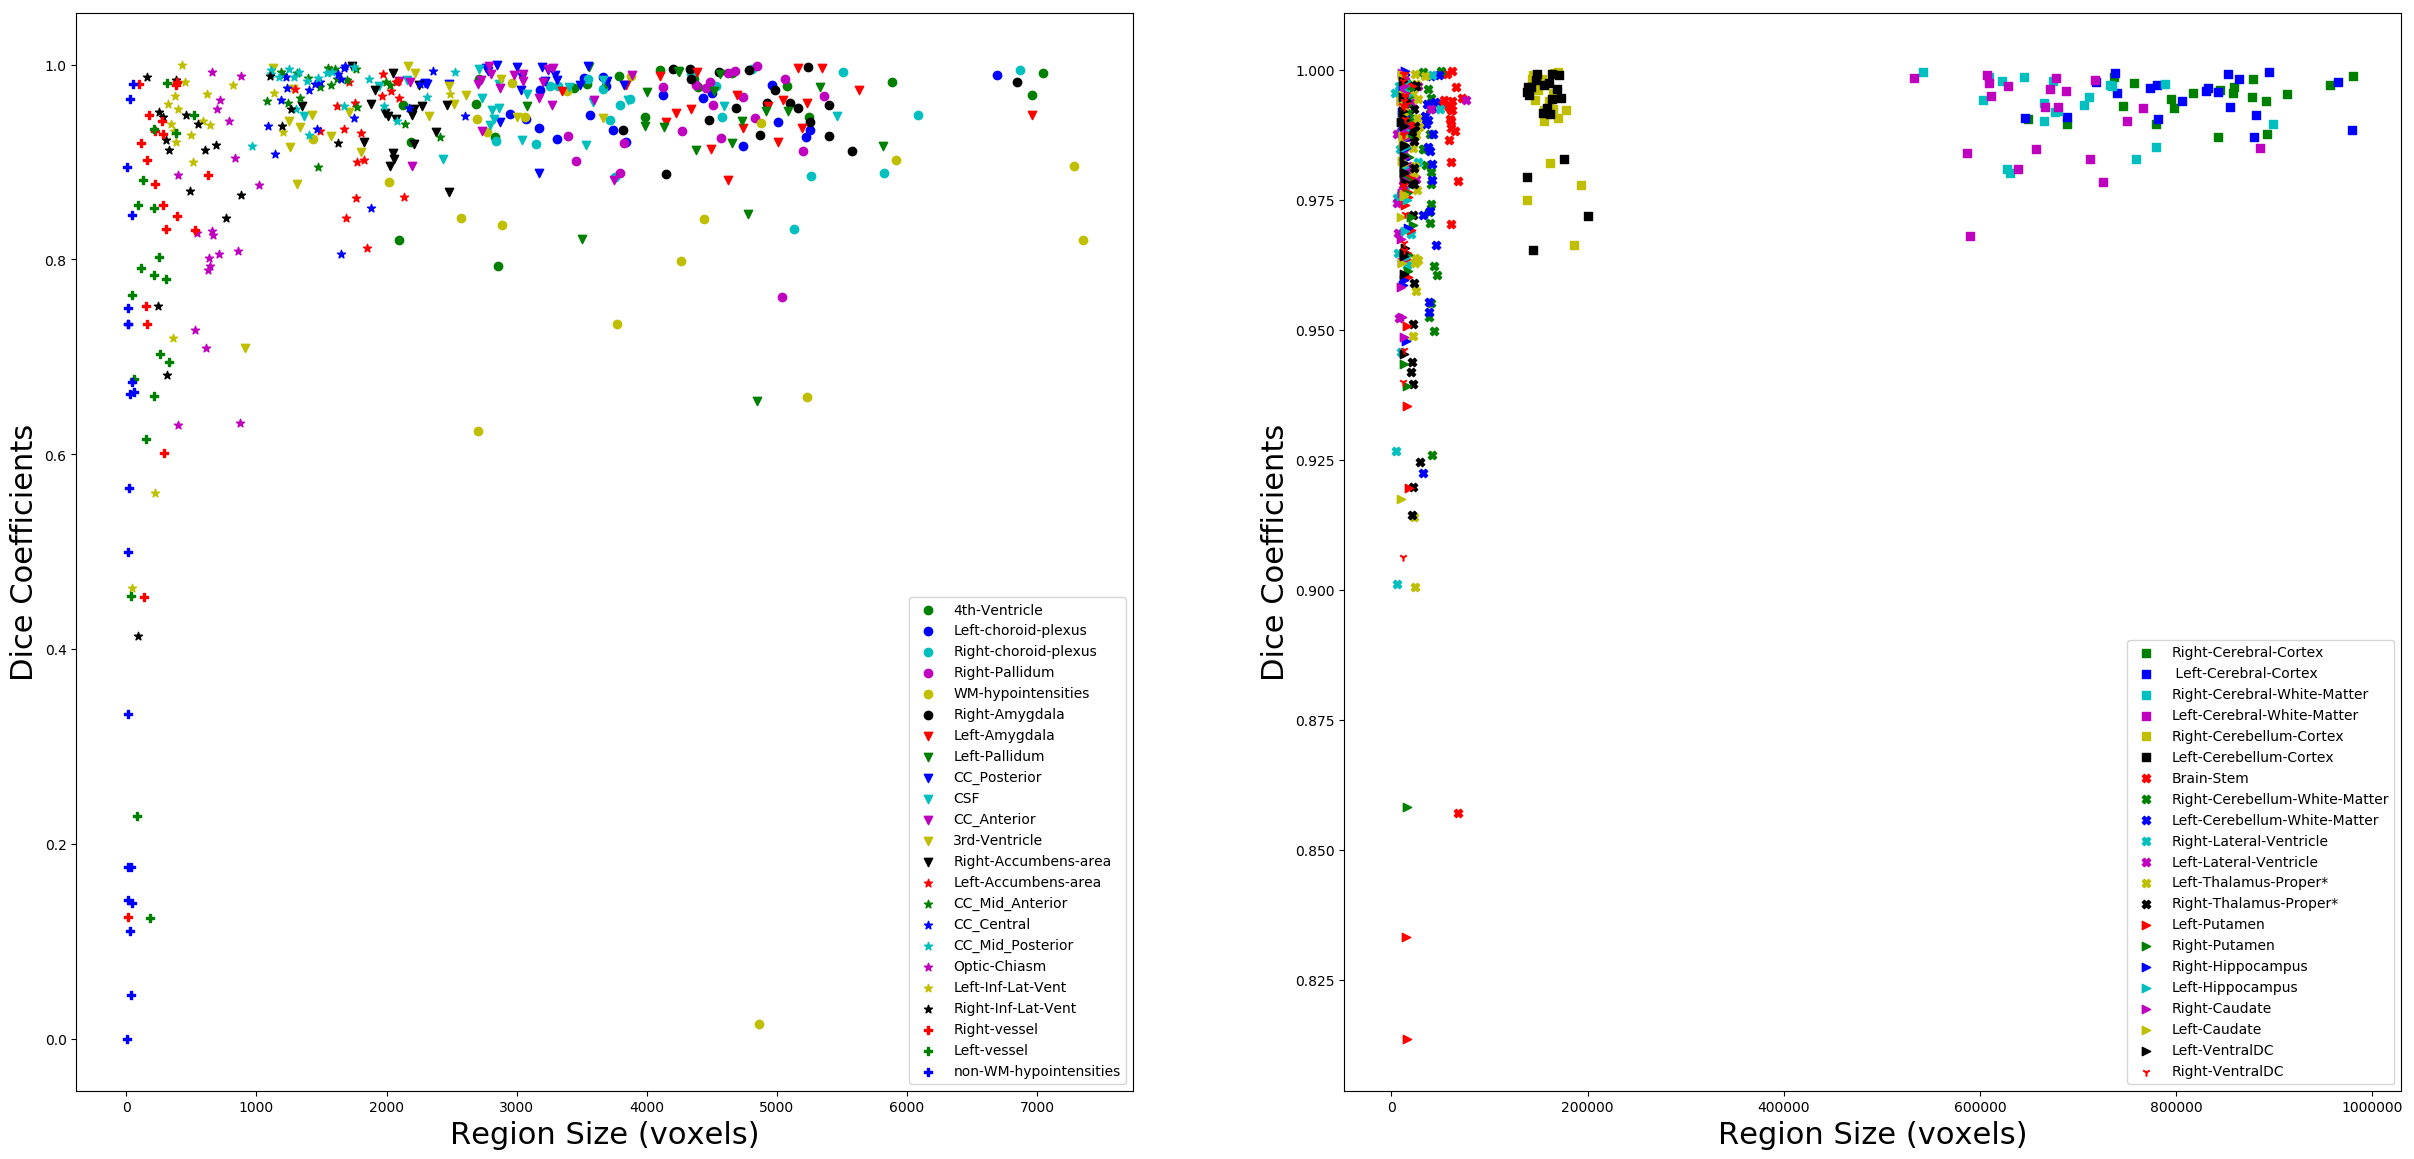
\includegraphics[width=\textwidth]{images/scatter_plot.png} 
    \caption{The scatter plots of the Dice coefficients between segmented regions 
            from 20 subjects in FreeSurfer (CentOS6 vs. CentOS7). 
            The x-axes are the number of voxels in each region and 
            y-axes are Dice values that are in different scales in two plots.
            The right plot shows the similarity between regions larger than $10^4$ voxels. 
            The left plot represents the differences between 
            regions smaller than $10^4$ voxels.
            The complete table of Dice coefficient values is 
            \href{https://github.com/ali4006/HCP-reproducibility-paper/blob/master/data/dice_values.csv}
            {available}.} 
    \label{fig:scatter_plot}
  \end{figure*}

  % We formulated the linear regression model for the Dice and region size variables as:
  % \[D=1 + T\epsilon ;    T=\frac{-1}{\overline{R}}\]
  % It is easier to obtain high overlaps with large regions, 
  % while smaller regions are harder to be similarly segmented.
  % We obtained the epsilon value of $\approx$ 8.3 voxels ($\approx$ 3mm) which indicate the minimum number
  % of voxels in each region that needs to be segmented.
  

\section{Discussion}

Method:
* we assume no concurrent file accesses.

* we assume that the provenance graph is oriented, i.e., a process cannot read or write in the same file. Reasonnable in general but wouldn't work 
for, say, out of core computations.

Comment on the overhead, number of executions (3, 2 in condition 1, 1 in condition 2)

Applicability: no instrumentation required, fast.
But not able to capture dependencies in memory.

We identified four processes that create differences 
among all 28 distinct processes that are involved in the PreFreeSurfer execution. 
The numerical instability in the 
PreFreeSurfer HCP pipeline arises mainly from linear 
registration processes implemented in FSL \emph{FLIRT}. 
We can see that \emph{FLIRT} creates differences in almost all the sub-pipelines. 
We monitored the library system calls using \emph{ltrace} to check that registration processes
use the same libraries. There were no differences in the library dependencies used by 
the tool in two operating systems, but we found a different number of calls to the \emph{glibc}.

In the second experiment, 
the analyses obtained by the FreeSurfer show substantial between-OS differences.
These results show the sensitivity of the segmentation process to the 
size of regions, however, it might be also sensitive to the location and shape of 
the segmented regions.
We demonstrate that static build of the pipeline would not improve the numerical stability of the pipeline. 
FreeSurfer pipeline propagates and amplifies the numerical differences that are created by the 
differences in the underlying operating system libraries.
These results are consistent with the findings in the paper~\cite{Glatard2015}, 
as it has confirmed the propagation of differences in cortical thickness extraction analysis using FreeSurfer.

We obtained results between OS versions; further investigations could be done over the OS families (e.g., Linux VS. Windows).
In addition to variations of the operating system, numerical instability of the pipelines have been 
explored when varying software, hardware and implementation details, or even by adding negligible 
perturbations like one voxel noise in the input dataset.
In the field of numerical analysis, we can investigate these issue using the Monte Carlo Arithmetic (MCA), 
a method instrumenting floating-point operations based on the random rounding algorithms at a target precision.
By this algorithm, we can locate the instabilities for the given pipelines, tools, or operations.

We demonstrate that computational models in neuroimaging are sensitive to numerical instabilities. 
Although we identify the processes in the pipeline that create differences, 
the amplification of these differences should be quantified in the future works.
We can use distance-preserving hashes rather than MD5 checksums or metrics specific to the file type like the Dice coefficient 
for the registration and segmentation processes to measure the magnitude of differences. 

% mention fuzzy libmath as a way to do this across distributions.

\section{Conclusion}

Our technique can characterize the stability of the pipelines
automatically. We identified the leading causes of the between-OS differences as (1) the evolution 
of the math libraries over time and (2) the instability of the pipelines. 
There are two ways to tackle this problem. The easy but less preferred solution is masking the instabilities.
This can be done by using, (1) single operating system for the processing of subjects, 
(2) containerizing the pipelines so that the 
processing is done on a more controlled environment, 
(3) increasing the numerical precision of the arithmetics, 
(4) building static executables by removing the host operating system library dependencies. 
These solutions only make the problem invisible, but the pipelines are still unstable.

\note{The preferred solution is to find the origin of amplification of differences and 
then fixing the particular functions/modules in the processing pipelines. 
Bagging is a fundamental technique toward reducing the instability of the analysis.
Therefore, we can use bagging for the parts in the pipeline that amplify differences, 
but it still is computationally expensive. }

% importance of data-driven evaluations, subject clustering, etc

% future work with MCA

% link registration to our motion estimation study

\section{Acknowledgments}

This research was enabled in part by support provided by 
Calcul Quebec (http://www.calculquebec.ca) and 
Compute Canada (http://www.computecanada.ca).
Also, data were provided by the Human Connectome Project, WU-Minn 
Consortium (Principal Investigators: David Van Essen and Kamil Ugurbil; 
1U54MH091657) funded by the 16 NIH Institutes and Centers that support 
the NIH Blueprint for Neuroscience Research; and by the McDonnell 
Center for Systems Neuroscience at Washington University.


% \begin{figure*}
% \centering
%   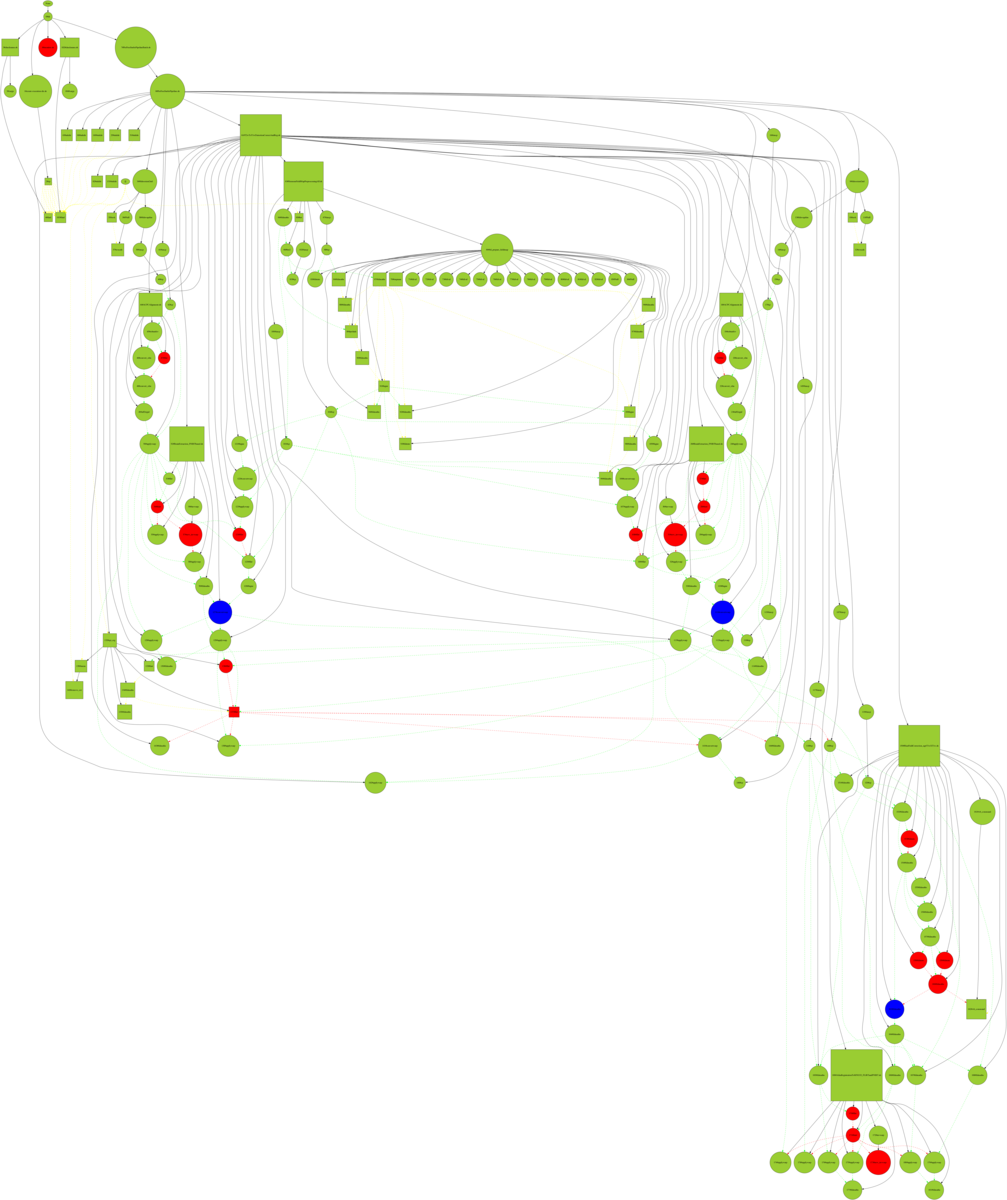
\includegraphics[width=.9\textwidth]{images/graph}
%   \caption{A complete process graph from the PreFreeSurfer pipeline.
% Full-resolution image available at \url{https://drive.google.com/open?id=174yyn8SuVOUcK5aRVw0bagjDanLD0FLt}.}
%   \label{fig:complete-graph}
% \end{figure*}

% \begin{figure*}
% \centering
%   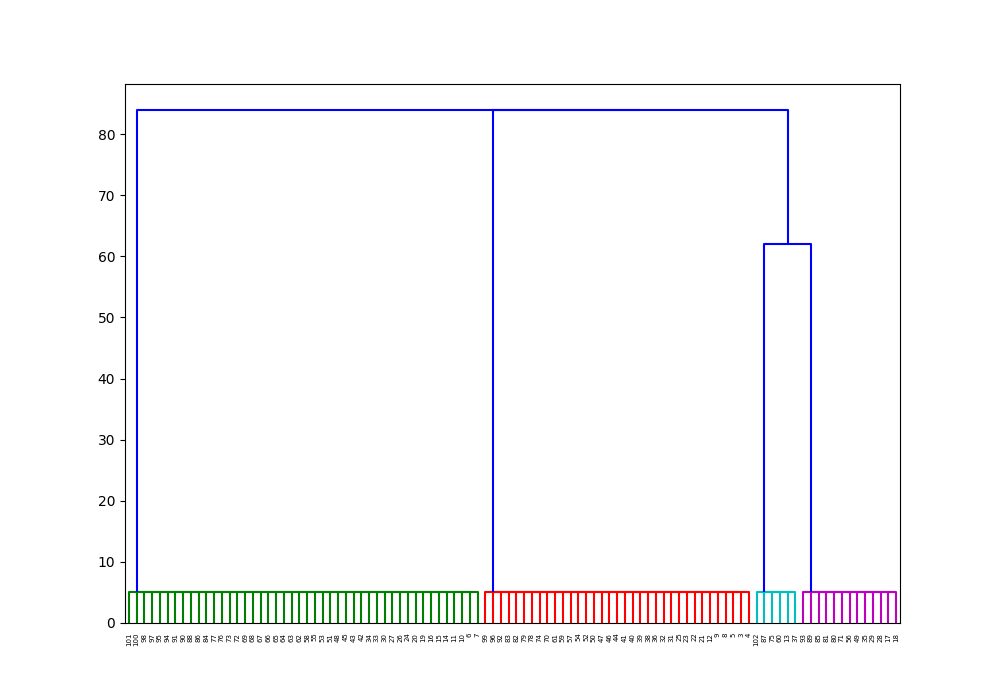
\includegraphics[width=.8\textwidth]{images/hclusters}
%   \caption{Different data types clustered among 100 subjects.}
%   \label{fig:subj-clusters}
% \end{figure*}



\bibliographystyle{plain}
\bibliography{biblio}


\end{document}
